\section{Motivation} \label{sec:motiv}

As we mentioned earlier, general purpose cores are highly inefficient 
and are optimized for single thread workloads only. They have very low energy efficiency
for server workloads mainly due to high-frequency, deep  pipelines, speculation
and explicit memory/register based communication~\cite{gpp_innef}.
Even the new heterogeneous offload engines like GPUs,FPGAs and ASICs face either 
programming or power-area challenges. So, this motivates us to
invent new heterogeneous offload engines which - i) achieves better scalability
and higher performance per watt, ii) have flexible programmer abstraction and
iii) able to target different program behaviors in the core regions -- both regular and irregular.  

With such requirements, this section tries to motivate why this type of architecture and programming abstraction
is needed for Proximate, and what are some of the insights and mechanisms needed to arrive 
at such architecture for current parallel workloads. 

\subsection{Insights}
The main insight for parallelization in Proximate is that - it
is reasonable to presume that programmer can reason about the
data/task locality of the kernel. Programmer managed data sharding
and task/data co-location is fairly straight forward for several server class
workloads. 
By co-locating the data and task you would reduce the access latency and 
achieve higher memory or cache bandwidth. 

The other insight we had was, each program or application can have multiple phases
during the program execution~\cite{nowatzki2016analyzing}. So, your
parallel hardware must be able to recognize such phases and offload the kernel to
corresponding hardware in a heterogeneous environment. Program regions generally tend to 
exhibit two main behaviors - i) Irregular data access pattern with low ILP and
ii) Regular data access patterns with high DLP. So, the architecture executing such programs need to
accelerate both these regions and the insight is to execute both these phases in proximate.
The final insight is that, since regular workloads are memory streaming workloads, the architecture needs
to support high bandwidth memory hierarchy and should be able to provide sufficient memory bytes in less number of cycles. 

\subsection{Mechanisms to Exploit Insights}

We now explain some of the mechanisms we have come up with to exploit the 
insights described above. 
\paragraph{Programmer Control Data/Task Locality}
The high level question one has to ask in how to give the programmers control
of data and task locality within proximate cores. We answer this
in Proximate by providing a flexible programming model to enable the 
programmer managed data sharding and task/data co-location. 
Figure~\ref{fig:prog-overview} shows the programmer's view of the architecture, 
and the vault abstraction proximate provides. Each vault is group of cores
and a predetermined slice of virtual address spaces, exposed during task offloading 
and memory allocation. 

\begin{figure}
  \begin{center}
    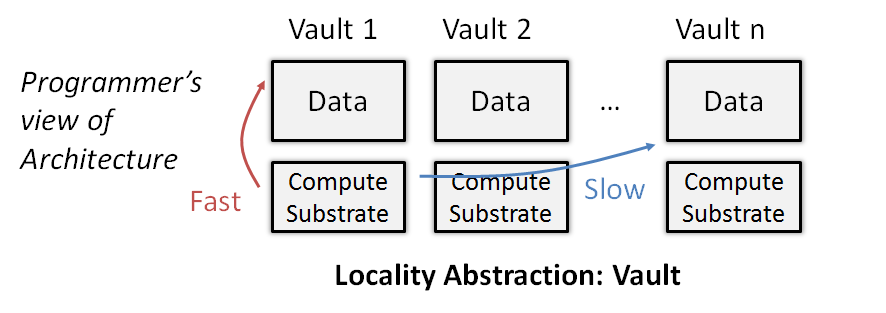
\includegraphics[width=\linewidth]{cs758-figs/prog-abs.png}
  \end{center}
\vspace{-0.2in}
  \caption{Programmer Abstraction of the Architecture}
  \label{fig:prog-overview}
\vspace{-0.05in}
\end{figure}


The locality abstraction for programmers is given by the vault. Each vault, 
has an address partition (data) and the compute substrate to work or offload task
on that address partition. There is a latency penalty if each compute substrate does an 
out-of-vault access to access data not in its address partition. By giving this abstraction to 
programmer, he/she can manage the data sharding explicitly and reason about the data/task locality.

\paragraph{Program Regions and Memory Bandwidth Requirement}To satisfy the high bandwidth demand and memory requirement, Proximate has address partitioned
per-vault caches. Proximate has simple in-order cores to target program regions exhibiting irregular data access patterns with low ILP. 
It has a high throughput compute engine (Softbrain) to target program regions exhibiting regular data access patterns with high DLP.
